%%%%%%%%%%%%%%%%%%%%%%%%%%%%%%%%%%%%%%%%%%%%%%%%%%%%%%%%%%%%%%%%%%%%%%%%%%%%
% AGUJournalTemplate.tex: this template file is for articles formatted with LaTeX
%
% This file includes commands and instructions
% given in the order necessary to produce a final output that will
% satisfy AGU requirements, including customized APA reference formatting.
%
% You may copy this file and give it your
% article name, and enter your text.
%
%
% Step 1: Set the \documentclass
%
%

%% To submit your paper:
\documentclass[draft]{agujournal2019}
\usepackage{url} %this package should fix any errors with URLs in refs.
\usepackage{lineno}
\usepackage[inline]{trackchanges} %for better track changes. finalnew option will compile document with changes incorporated.
\usepackage{soul}
\linenumbers

%CMZ
\usepackage{natbib}
%\usepackage{xcolor}
\usepackage{graphicx}
\newcommand{\degree}{$^{\circ}$}
\newcommand{\texttilde}{$\sim$}


%%%%%%%
% As of 2018 we recommend use of the TrackChanges package to mark revisions.
% The trackchanges package adds five new LaTeX commands:
%
%  \note[editor]{The note}
%  \annote[editor]{Text to annotate}{The note}
%  \add[editor]{Text to add}
%  \remove[editor]{Text to remove}
%  \change[editor]{Text to remove}{Text to add}
%
% complete documentation is here: http://trackchanges.sourceforge.net/
%%%%%%%

\draftfalse

%% Enter journal name below.
%% Choose from this list of Journals:
%
% JGR: Atmospheres
% JGR: Biogeosciences
% JGR: Earth Surface
% JGR: Oceans
% JGR: Planets
% JGR: Solid Earth
% JGR: Space Physics
% Global Biogeochemical Cycles
% Geophysical Research Letters
% Paleoceanography and Paleoclimatology
% Radio Science
% Reviews of Geophysics
% Tectonics
% Space Weather
% Water Resources Research
% Geochemistry, Geophysics, Geosystems
% Journal of Advances in Modeling Earth Systems (JAMES)
% Earth's Future
% Earth and Space Science
% Geohealth
%
% ie, \journalname{Water Resources Research}

\journalname{Enter journal name here}


\begin{document}

%% ------------------------------------------------------------------------ %%
%  Title
%
% (A title should be specific, informative, and brief. Use
% abbreviations only if they are defined in the abstract. Titles that
% start with general keywords then specific terms are optimized in
% searches)
%
%% ------------------------------------------------------------------------ %%



\title{Differences in algorithmic rain-on-snow flood climatology across historical data products}

%% ------------------------------------------------------------------------ %%
%
%  AUTHORS AND AFFILIATIONS
%
%% ------------------------------------------------------------------------ %%

% Authors are individuals who have significantly contributed to the
% research and preparation of the article. Group authors are allowed, if
% each author in the group is separately identified in an appendix.)

% List authors by first name or initial followed by last name and
% separated by commas. Use \affil{} to number affiliations, and
% \thanks{} for author notes.
% Additional author notes should be indicated with \thanks{} (for
% example, for current addresses).

% Example: \authors{A. B. Author\affil{1}\thanks{Current address, Antartica}, B. C. Author\affil{2,3}, and D. E.
% Author\affil{3,4}\thanks{Also funded by Monsanto.}}

\authors{Colin M. Zarzycki\affil{1}, Benjamin D. Ascher\affil{1}\thanks{now at Colorado State University}, and Alan M. Rhoades\affil{2}}


\affiliation{1}{Penn State}
\affiliation{2}{LBNL}
% \affiliation{3}{Third Affiliation}
% \affiliation{4}{Fourth Affiliation}

%% Corresponding Author:
% Corresponding author mailing address and e-mail address:

% (include name and email addresses of the corresponding author.  More
% than one corresponding author is allowed in this LaTeX file and for
% publication; but only one corresponding author is allowed in our
% editorial system.)

% Example: \correspondingauthor{First and Last Name}{email@address.edu}

\correspondingauthor{Colin M. Zarzycki}{cmz5202@psu.edu}

%% Keypoints, final entry on title page.

%  List up to three key points (at least one is required)
%  Key Points summarize the main points and conclusions of the article
%  Each must be 100 characters or less with no special characters or punctuation and must be complete sentences

% Example:
% \begin{keypoints}
% \item	List up to three key points (at least one is required)
% \item	Key Points summarize the main points and conclusions of the article
% \item	Each must be 100 characters or less with no special characters or punctuation and must be complete sentences
% \end{keypoints}

\begin{keypoints}
\item enter point 1 here
\item enter point 2 here
\item enter point 3 here
\end{keypoints}

%% ------------------------------------------------------------------------ %%
%
%  ABSTRACT and PLAIN LANGUAGE SUMMARY
%
% A good Abstract will begin with a short description of the problem
% being addressed, briefly describe the new data or analyses, then
% briefly states the main conclusion(s) and how they are supported and
% uncertainties.

% The Plain Language Summary should be written for a broad audience,
% including journalists and the science-interested public, that will not have 
% a background in your field.
%
% A Plain Language Summary is required in GRL, JGR: Planets, JGR: Biogeosciences,
% JGR: Oceans, G-Cubed, Reviews of Geophysics, and JAMES.
% see http://sharingscience.agu.org/creating-plain-language-summary/)
%
%% ------------------------------------------------------------------------ %%

%% \begin{abstract} starts the second page

\begin{abstract}
[ enter your Abstract here ]
\end{abstract}

\section*{Plain Language Summary}
[ enter your Plain Language Summary here or delete this section]


%% ------------------------------------------------------------------------ %%
%
%  TEXT
%
%% ------------------------------------------------------------------------ %%

%%% Suggested section heads:
% \section{Introduction}
%
% The main text should start with an introduction. Except for short
% manuscripts (such as comments and replies), the text should be divided
% into sections, each with its own heading.

% Headings should be sentence fragments and do not begin with a
% lowercase letter or number. Examples of good headings are:

% \section{Materials and Methods}
% Here is text on Materials and Methods.
%
% \subsection{A descriptive heading about methods}
% More about Methods.
%
% \section{Data} (Or section title might be a descriptive heading about data)
%
% \section{Results} (Or section title might be a descriptive heading about the
% results)
%
% \section{Conclusions}


\section{= enter section title =}
%Text here ===>>>


While RoS events have been impressively this work has overwhelmingly focused on mountainous regions \citep{singh1997hydrological,mccabe2007rain,musselman2018projected} there has been less focus on compound snowmelt-flooding extremes in areas with more ephemeral snow cover, even though these events are key drivers of `slow-rise' flooding in the northeastern quadrant of the United States that peaks in late winter and spring \citep{ashley2008flood,villarini2010flood,dougherty2019climatology}.





A common misconception is that RoS events are generated by warm rain providing heat to the snowpack. Multiple studies have found that the actual heat transfer between the liquid rain and surface snowpack is rather small and explains a small fraction of the observed snowmelt \citep{moore1984controls}. Rather, work has shown that factors such as surface humidity and temperature (and associated latent and sensible heat fluxes) and downwelling radiation are key players \citep{wurzer2016influence,harpold2018humidity}.

In the northeastern United States, events such as the 1996 event are associated with a confluence of surface conditions, including anomalously high heat fluxes into the snow pack which are associated with stormy conditions.

Rapid snow ablation in regions with ephemeral snow have been shown to have a strong correlation with subsequent increases in basin streamflow. For example, \citet{suriano2020discharge} found that 75\% of snow ablation events in the SRB (defined by daily decrease in snow depth in above-freezing conditions) yielded increased river discharge three days later.





\citet{collins2014annual} found that mixed snowmelt and rainfall events were a key driver of flooding in New England and Atlantic Canada during late winter and early spring. \citet{wachowicz2020rain} produced a pointwise climatology of RoS events in the eastern United States using the dataset of \citet{dyer2006spatial}, finding the majority of RoS events in the region occurred in spring. \citet{grote2021synoptic} composited the synoptic meteorological fields of six recent RoS events in the mid-Atlantic region and found that flooding was driven by an inland-running extratropical cyclone that advected warm, moist air in the warm sector of the cyclone into the study region.

While climatological studies such \citet{wachowicz2020rain} are critically important, event-level analysis has become increasingly important for stakeholders \citep{shepherd2018storylines}. This becomes a complex challenge when working with gridded climate data, particularly for future model projections of which no observational reference exists. To extract information regarding singular extreme events and their corresponding statistics, algorithmic techniques which objectively analyze datasets without manual intervention need to be devised.

Here, we demonstrate a technique for generating an event database at the basin-scale in arbitrary climate datasets. We focus on the direct prediction of couple surface processes (i.e., snow water equivalent and surface runoff) to minimize issues with statistical or dynamical downscaling. 


XXXXXX

\section{Methods}

\subsection{Datasets}


To evaluate the suitability of historical products, we evaluate four products that seek to reproduce observed conditions, although each with a different form.

First, L15

Second, NLDAS-VIC4.0.5

Third, a full, global reanalysis JRA-55. Reanalyses are derived from running prognostic 3-D Earth system models while assimilating observational data as they are integrated. Therefore, they serve as a bridge between in-situ observational data and free-running climate models. More details re: reanalyses can be found in XXX.

Finally, a nudged version of the DoE E3SM model is run at 1\degree{} spatial resolution. This simulation is analogous to the majority of climate models in CMIP6. To constrain the large-scale meteorology to that observed, the simulation is nudged to ERA5 reanalysis at 6-hourly timescales, with acts as a crude assimilation technique. This nudging is performed above the boundary layer, which offers the advantage of reproducing patterns of 500 hPa geopotential height and sea level pressure while allowing the model to simulate grid-scale processes relatively freely \citep{sun2019impact}. While E3SM is run on an unstructured cubed-sphere mesh, the simulation output is regridded to a 1\degree{}x1\degree{} regular latitude-longitude mesh using higher-order methods \citep{hill2004architecture}. 

\subsection{Defining basin-scale events}

Three variables are extracted over the SRB. These include total precipitation (liquid and frozen, summed), surface snow water equivalent (SWE), and surface water runoff (ROF). All data is standardized to daily average values by temporally-averaging any subdaily (e.g., hourly) data at each grid cell. The SRB is defined using a shapefile (MORE INFO). Grid cells that have at least 50\% of their area enclosed by the boundary of the SRB are kept, while those exterior to the SRB ($<$50\%) are set to missing values. Results using a simple latitude-longitude box encompassing the SRB demonstrated similar results (not shown). A basin-wide timeseries is then constructed by spatially averaging the three fields for each calendar day (00Z to 00Z) and smoothing the resulting time series using a simple moving average to reduce day-to-day noise in the derived variables. We choose a 5-day window based on synoptic timescales \citep{holton2004introduction}, although perturbations to this averaging period didn't materially change any of the findings here. Rain-on-snow days are defined algorithmically by flagging coincident times of negative dSWE and surface runoff that both exceed certain thresholds in the smoothed SRB timeseries. We test two methods of thresholding; one uses fixed thresholds across all datasets (FIXED) and the other defines dataset specific thresholds by those exceeding 95\% (RELATIVE) over the dataset. For fixed thresholds, we require an average dSWE of -1.4 mm/day and surface runoff rate of 1.4 mm/day. Note that while the majority of the events are associated with precipitation (e.g., rain-on-snow) we do not exclude a specific precipitation criterion, but rather, leverage surface runoff as a proxy for surface flooding. The processing was verified by comparing the Pearson correlation of basin-wide statistics across all products. All permutations resulted in acceptably high correlations (greater than XXX, Table SX), confirming that all datasets adequately represent the historical time series.

\section{Results}

\subsection{Climatology}

The mean climatologies for all four products are shown in Fig. \ref{fig:means}. The mean precipitation r

The higher resolution nature of both the NLDAS and L15 products is also evident from the spatial structure in the mean fields.

It is well-known that simulated runoff from different hydrologic models can be extremely variable, with regional differences between products reaching an order of magnitude in some cases \citep{gudmundsson2012comparing,sood2015global,beck2017global}. 

While there is less product-to-product variability in precipitation and snow water equivalent (SWE), it has been found that significant spread still exists in climate data products even for precipitation.

Table \ref{table:means}. shows the 


\begin{figure}
\begin{tabular}{c}
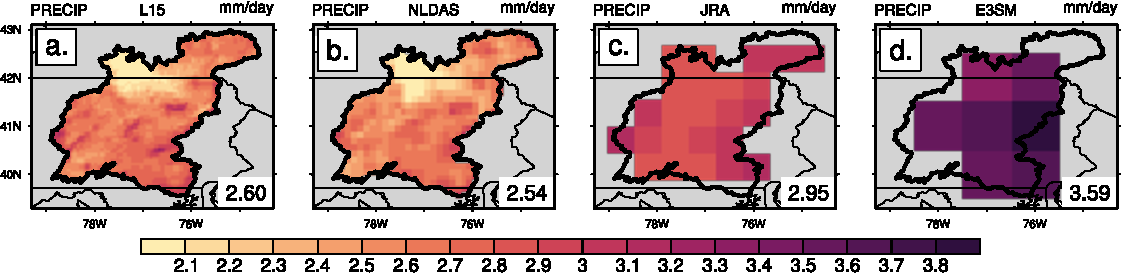
\includegraphics[width=0.98\linewidth]{{figs/cropped/climo_comp_panel_PRECIP}.pdf} \\
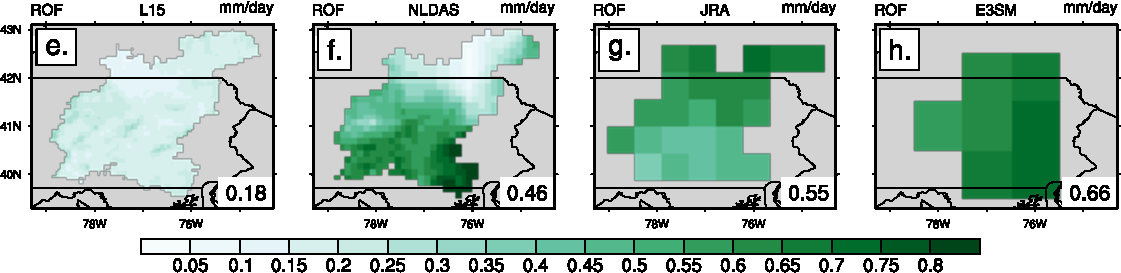
\includegraphics[width=0.98\linewidth]{{figs/cropped/climo_comp_panel_ROF}.pdf} \\
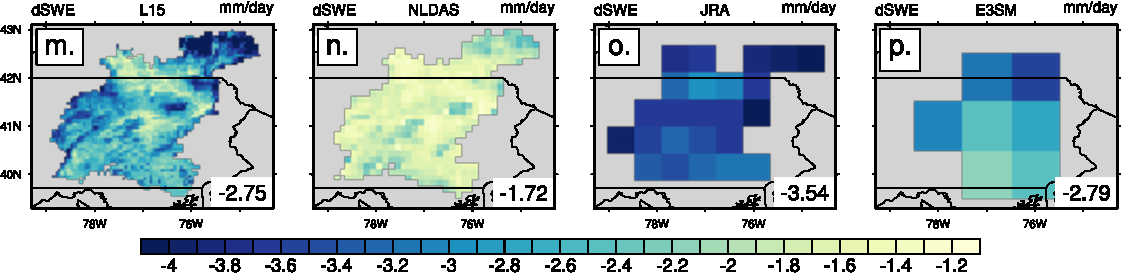
\includegraphics[width=0.98\linewidth]{{figs/cropped/climo_comp_panel_dSWE}.pdf} \\
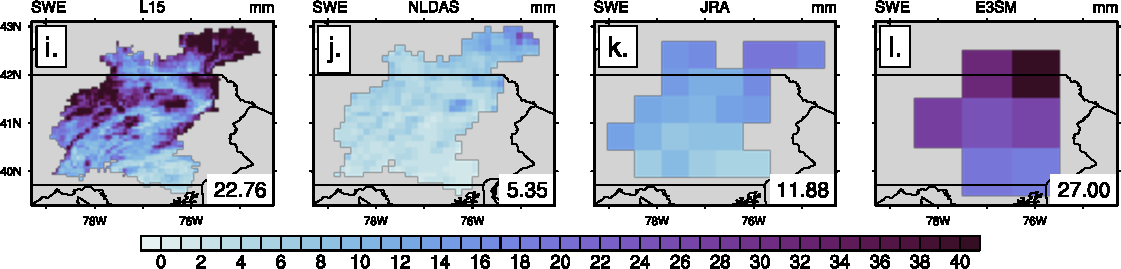
\includegraphics[width=0.98\linewidth]{{figs/cropped/climo_comp_panel_SWE}.pdf}
\end{tabular}
\caption{....}
\label{fig:means}
\end{figure}


\begin{table}
\resizebox{\textwidth}{!}{%
\begin{tabular}{lllllllllll}
                & ROS\_t & dSWE\_t & Events & Duration & dSWE & dSWE\_max & ROF & ROF\_max & Precip & Precip\_max \\
RELATIVE (95\%) &        &         &        &          &      &           &     &          &        &             \\
E3SM            & 1.78   & 2.22    & 42     & 4.6      & 6.9  & 8.5       & 2.6 & 3.0      & 6.1    & 7.3         \\
JRA             & 1.57   & 1.85    & 40     & 3.2      & 4.0  & 5.1       & 2.6 & 2.9      & 5.4    & 6.1         \\
L15             & 0.62   & 1.49    & 20     & 6.0      & 4.8  & 6.1       & 0.9 & 1.1      & 5.4    & 6.8         \\
NLDAS           & 1.42   & 0.79    & 21     & 2.9      & 3.2  & 3.8       & 1.9 & 2.0      & 6.1    & 6.7         \\
                &        &         &        &          &      &           &     &          &        &             \\
FIXED           &        &         &        &          &      &           &     &          &        &             \\
E3SM            & 1.40   & 1.40    & 60     & 4.6      & 5.2  & 6.8       & 2.2 & 2.6      & 5.8    & 7.1         \\
JRA             & 1.40   & 1.40    & 48     & 3.5      & 3.5  & 4.7       & 2.5 & 2.8      & 5.3    & 6.1         \\
L15             & 1.40   & 1.40    & 6      & 3.2      & 6.8  & 7.5       & 1.6 & 1.7      & 8.6    & 9.1         \\
NLDAS           & 1.40   & 1.40    & 17     & 3.0      & 3.8  & 4.5       & 1.9 & 2.0      & 5.8    & 6.4        
\end{tabular}
}
\caption{....}
\label{table:means}
\end{table}

The differences between the datasets can be more readily noted in Figure \ref{fig:histograms}. All panels show statistics using the `relative' method where the algorithm thresholds are re-calibrated for each dataset. Fig. Xa. shows total number of events flagged over the time period, while Figs. Xb.-d. show the binned probabilities of daily maximum event-level precipitation, runoff, and change in SWE, respectively. All values are basin averages. The maximum precipitation associated with events is relatively similar between the four data products, with E3SM tending to have slightly more extreme precipitation occurring over the basin during the events flagged in that dataset (in agreement with Fig. \ref{fig:means}). Larger differences are seen in runoff and dSWE. In runoff, both the E3SM and JRA datasets produce larger magnitudes of surface runoff (i.e., flooding) compared to the other two datasets. L15 produces events with the least surface runoff (averaging approximately one-third of that in E3SM and JRA), with NLDAS lying between all three. The PDF of dSWE paints an even more complex picture, with 

Taken above, in either a relative or fixed threshold configuration, the 3-D coupled products (E3SM and JRA) produce more rain-on-snow events than L15 and NLDAS. While daily precipitation in each product differs somewhat, it should be noted that these differences are relatively small and precipitation is not actually used to flag RoS events. Rather, in our algorithm, majority of the difference in RoS events flagged across the datasets arises from lower magnitudes of runoff (dSWE) in the L15 (NLDAS) dataset. It is worth noting that L15 and NLDAS produce fewer RoS events regardless of which thresholding is used, so not only is the distribution of relevant daily variables shifted relative to the other models, but that the skewness is impacted as well.

\begin{figure}
\begin{tabular}{cc}
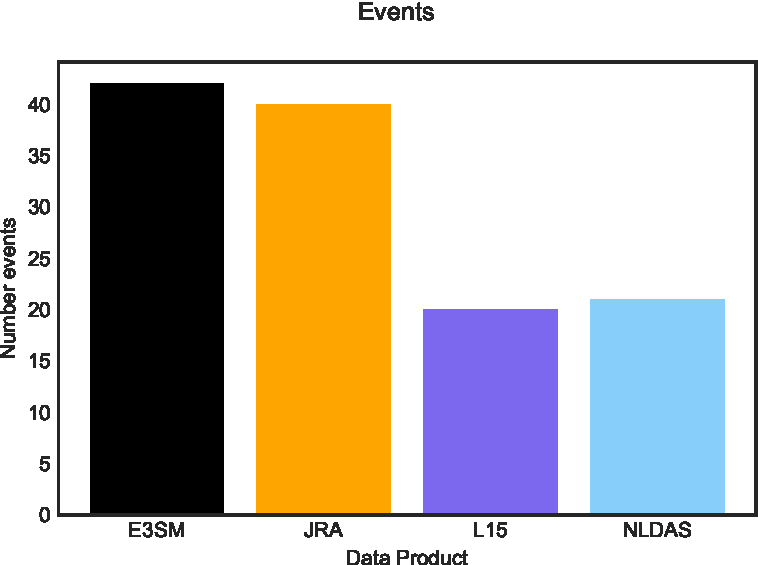
\includegraphics[width=0.45\linewidth]{{figs/cropped/events}.pdf} & 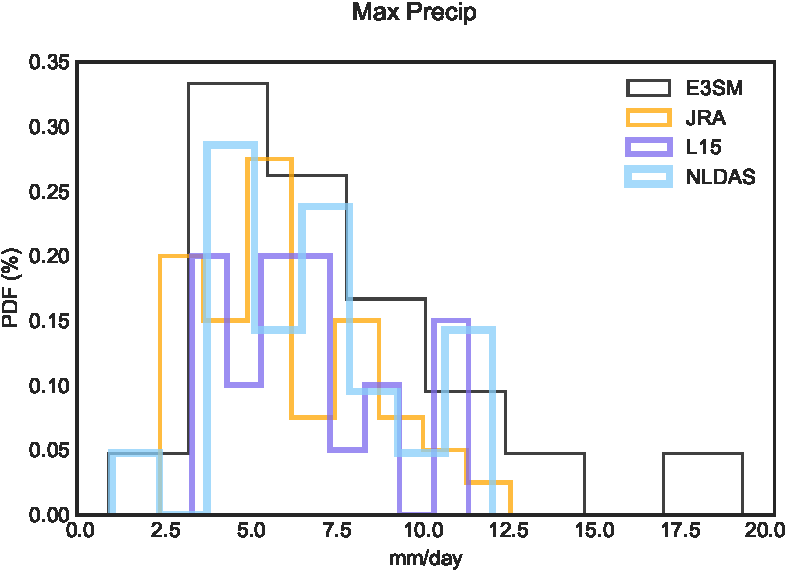
\includegraphics[width=0.45\linewidth]{{figs/cropped/Max_precip}.pdf} \\
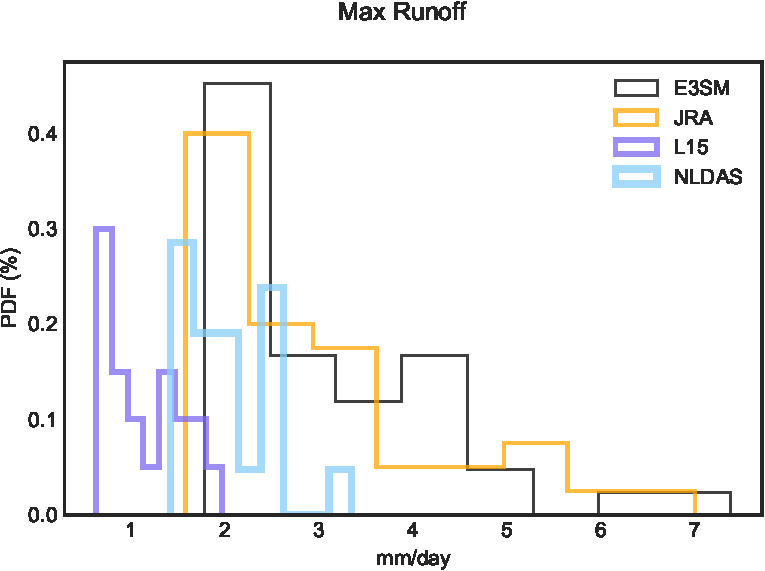
\includegraphics[width=0.45\linewidth]{{figs/cropped/Max_runoff}.pdf} & 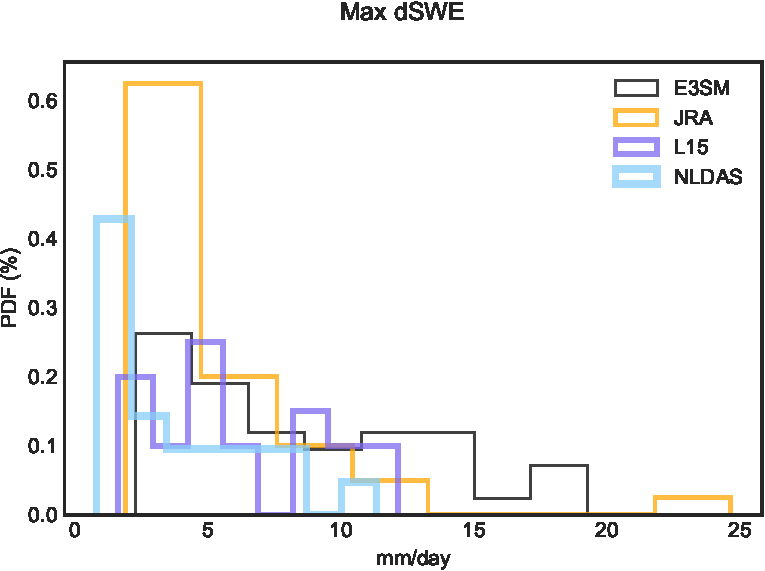
\includegraphics[width=0.45\linewidth]{{figs/cropped/Max_dSWE}.pdf}
\end{tabular}
\caption{....}
\label{fig:histograms}
\end{figure}

\subsection{Single-year evaluation}

\begin{figure}
\begin{tabular}{cc}
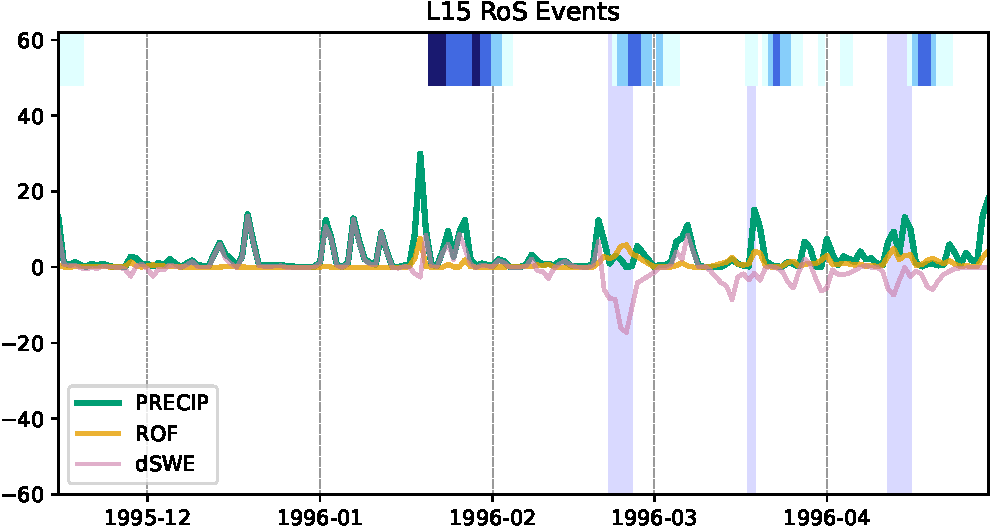
\includegraphics[width=0.45\linewidth]{{figs/cropped/L15_1995_events}.pdf} & 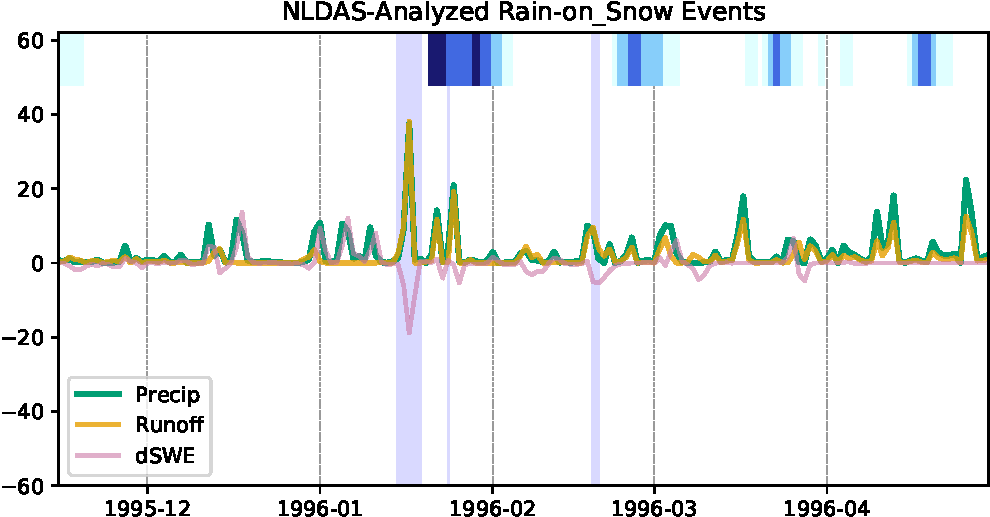
\includegraphics[width=0.45\linewidth]{{figs/cropped/NLDAS_1995_events}.pdf} \\
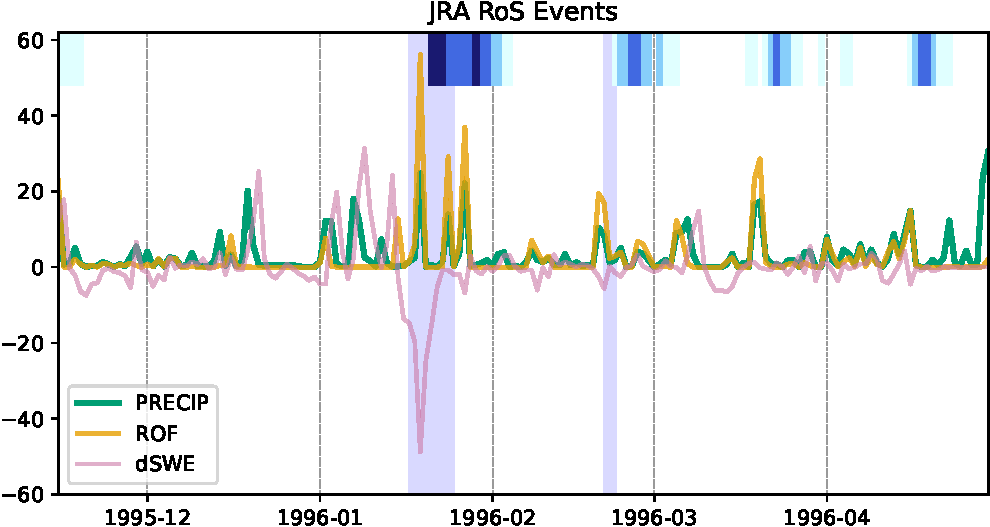
\includegraphics[width=0.45\linewidth]{{figs/cropped/JRA_1995_events}.pdf} & 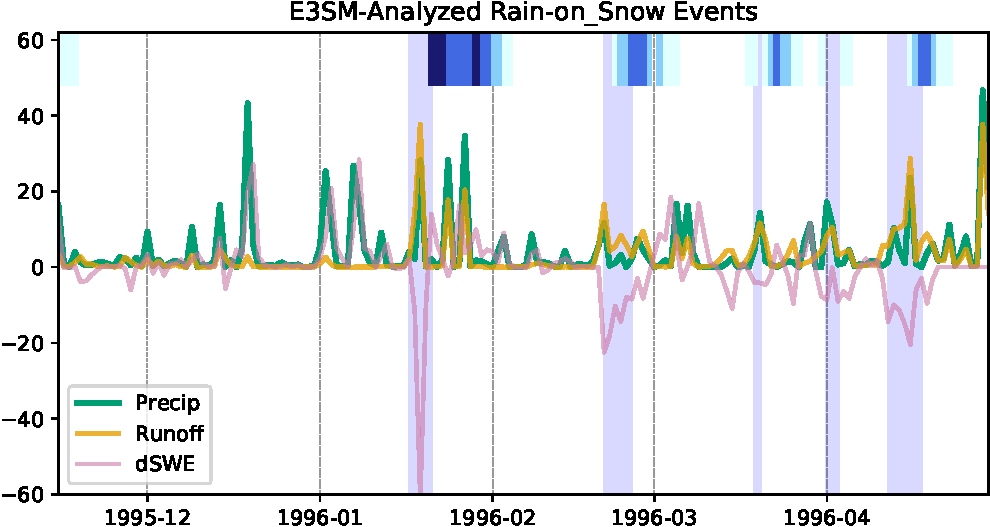
\includegraphics[width=0.45\linewidth]{{figs/cropped/E3SM_1995_events}.pdf}
\end{tabular}
\caption{....}
\label{fig:yr-timeseries-comp}
\end{figure}

\begin{figure}
\begin{tabular}{cc}
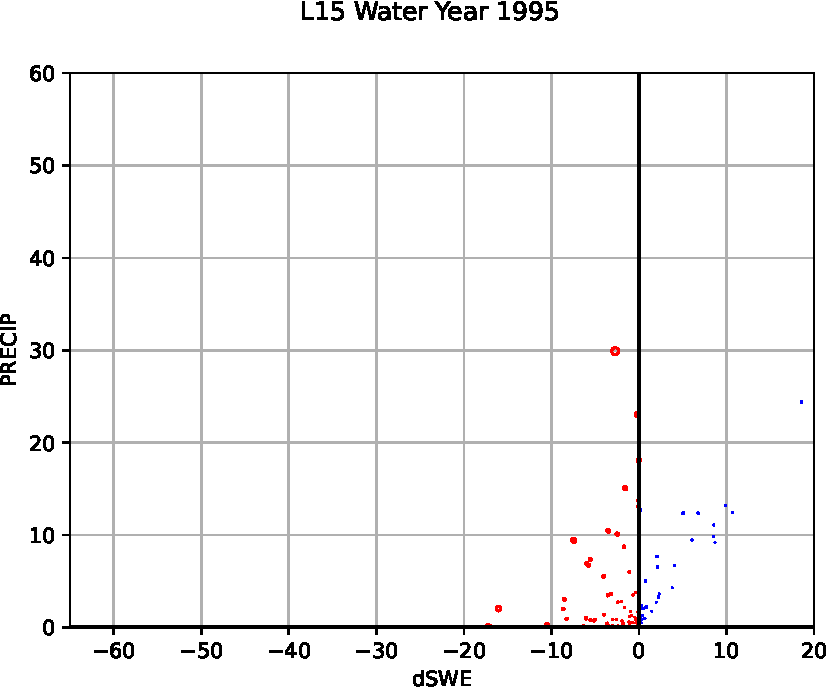
\includegraphics[width=0.45\linewidth]{{figs/cropped/L15_1995_scatplot}.pdf} & 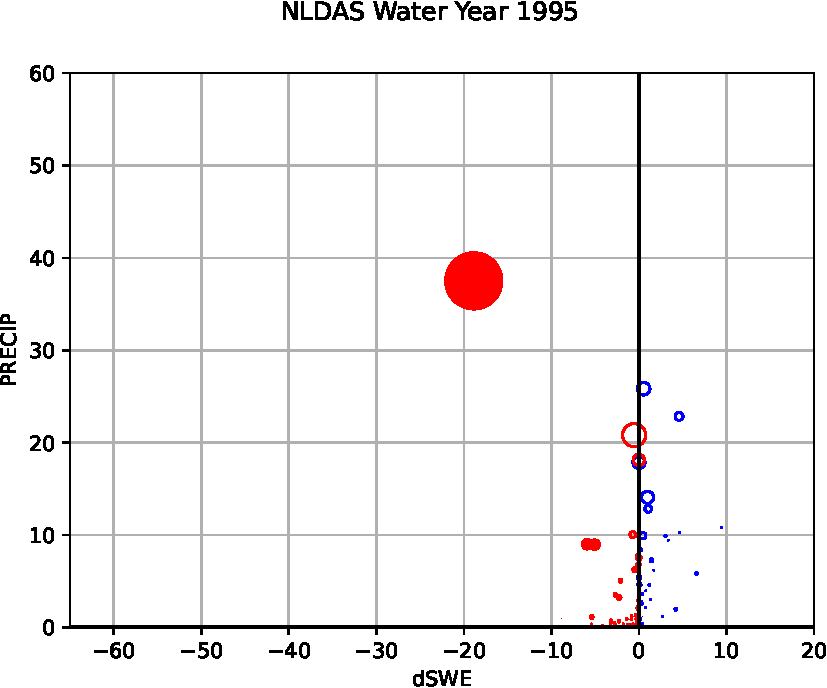
\includegraphics[width=0.45\linewidth]{{figs/cropped/NLDAS_1995_scatplot}.pdf} \\
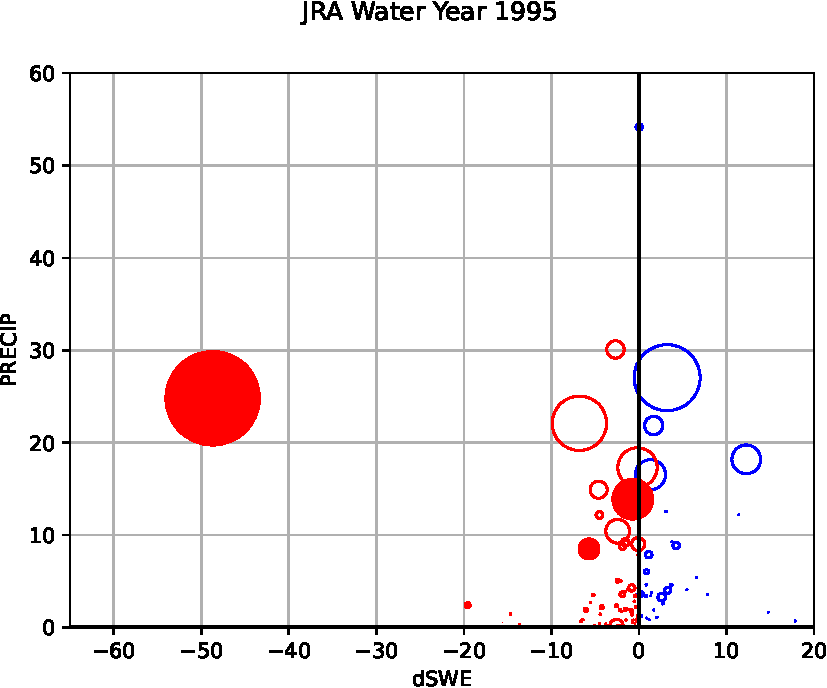
\includegraphics[width=0.45\linewidth]{{figs/cropped/JRA_1995_scatplot}.pdf} & 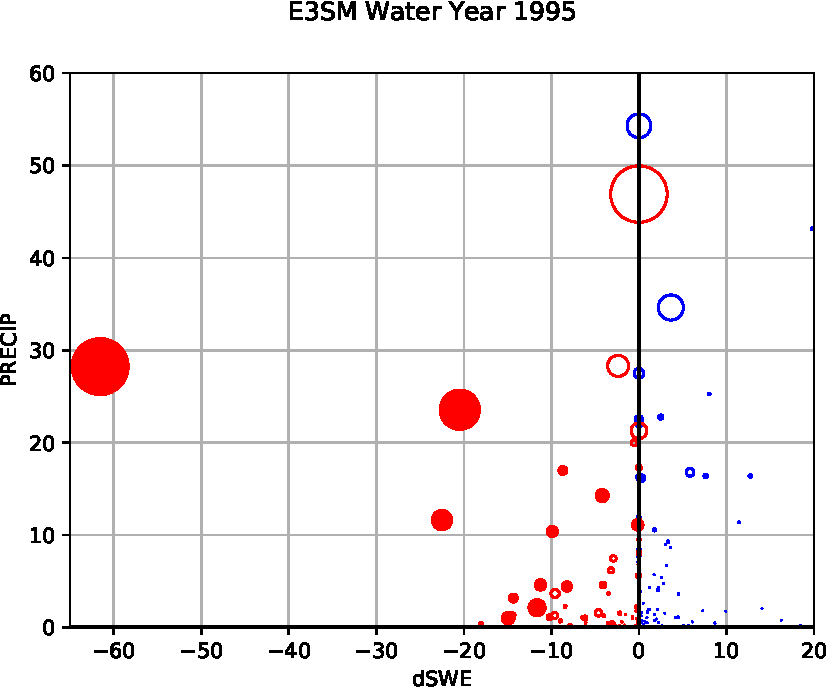
\includegraphics[width=0.45\linewidth]{{figs/cropped/E3SM_1995_scatplot}.pdf}
\end{tabular}
\caption{....}
\label{fig:bubble-comp}
\end{figure}

To further explore the event climatology at a more granular level, we focus on results associated with a single water year across all datasets. In particular, we choose the 1995 water year (WY95, September 1995 to August 1996) since this includes the 1996 rain-on-snow floods over the SRB \citep{leathers1998severe}.

Fig. \ref{fig:yr-timeseries-comp} shows the daily WY95 time series of basin-integrated PRECT, ROF, and dSWE for all four products. Negative (positive) dSWE denotes snow melt (accumulation). Shaded are events that were flagged by the snowmelt algorithm to be important. Also shown at the top is a stripe with four different gradient shadings, representing days of 75\%, 90\%, 95\%, and 99\% streamflow for United States Geological Survey (USGS) gauge data at Harrisburg, PA (USGS \#01570500), with darker colors representing anomalously high flow conditions.

The 1996 event is readily apparent in Mid-January, with three of the four products noting increases in precipitation and runoff and large SWE losses. Observed streamflow spiked during and immediately after the event as shown by the dark blue stripes at the top of each timeseries, indicated prolonged periods of observed daily streamflow exceeding the 99th percentile. While this is the largest RoS event observed over the 1985-2005 period, there remains large discrepancies between the four products. The snow loss signal is largest in magnitude for JRA and E3SM compared to NLDAS. L15 shows a very minimal SWE loss, to the point that the event thresholds are not triggered to classify this as a RoS event in that dataset. Precipitation is more similar across the three datasets, implying that the reduced surface runoff in L15 is due to the lack of snow ablation rather than the lack of rainfall.

All four products also indicate a second, more moderate RoS event over the SQ during the last third of February, although L15 and E3SM show larger dSWE signals and JRA and E3SM show larger runoff signals than the other two products. Streamflow exceeded the 95th percentile for this event, as shown by the striping at the top of each panel. More moderate flooding appears to occur in March and April, although only L15 and E3SM flag these as events by the algorithm definition. The fact that all events in all datasets flagged by the algorithm result in well-above-average streamflow lends credence to the efficacy of capturing hydrologically important atmosphere-land extremes.

Another way to visualize the WY95 data is shown in Fig. \ref{fig:bubble-comp}.  This plot shows the daily distribution of all three quantities by plotting dSWE on the x-axis, PRECIP on the y-axis, and the size of the x-y marker depicting the magnitude of the surface runoff. Markers are filled if the RoS criteria is triggered for that calendar day and are colored red (blue) if there is SWE loss (gain). The variability of the precipitation (y-axis) is the most similar between models, with the vast majority of daily basin-scale precipitation remaining below 30 mm/day, although E3SM produces a few days with more extreme precipitation rates, in agreement with E3SM being a slightly ``wetter'' products. Larger differences are noted the other two metrics. There is wide spread along the y-axis for JRA and E3SM, indicating that the coupled climate system models produce days with larger magnitudes of SWE changes. Further, L15 has markers that are small in size, indicating low daily surface runoff magnitudes when compared to the other three products. It is clear that there is substantial spread across the datasets, even when predicting the same timeseries, particular days further away from the 0,0 point.


\section{Discussion}

Here, we interrogate four different datasets that include daily information regarding precipitation, surface runoff, and snow water equivalent in order to quantify differences in how datasets might represent coupled land-atmosphere processes over the historical record. In particular, we focus on rain-on-snow floods over the Susquehanna. Flagging for periods of collocated runoff and dSWE does a reasonable job of marking periods that will be followed by climatologically above-normal streamflow in the basin. We find that using fixed thresholds across multiple datasets leads to large discrepancies in event frequency over the historical period, a factor of 10 between the most active and least active products. Normalizing these thresholds by each product's internal daily distribution improves agreement, although there remains approximately a factor two difference between event counts, implying that the underlying distributions in the reforecast land surface are fundamentally different in both shape and magnitude.

Interestingly, although we refer to these events as RoS events, there is no explicit precipitation requirement in the algorithm. However, we find that 75\% of events have at least one day of greater than 5 mm/day of basin-averaged precipitation and 95\% have at least one day of measurable precipitation as defined as greater than 1 mm/day. This implies that while ablation-only events can lead to rapid snowmelt, the vast majority of events producing large surface flooding signals involve some form of atmospheric precipitation as well. It also underscores the complex assessment of such flood events -- while rainfall onto an existing snowpack is not a primary driver of melt \citep{harpold2018humidity}, the common synoptic meteorological patterns \citep{grote2021synoptic} and additional liquid input to the surface (i.e., runoff being a combination of snowmelt and water flux from the atmosphere) leads to the majority of flood events being associated with at least some precipitation.

How data is generated for forcing is critically important. Since RoS events in regions of ephemeral snow (e.g., SQ) can have surface forcing at hourly timescales (e.g., XXXXXX), using daily meteorological data (as in NLDAS and L15) to force offline LSMs will likely underpredict RoS frequency. This occurs because time-interpolated data (and less frequent coupling) clips short-term extrema and risks offsetting the required superposition of multiple anomalies (e.g., high temperature, extreme rainfall) required to accurately simulate short-term extremes. Even at lower spatial resolutions, models coupled at shorter timescales (e.g., reanalysis, nudged coupled GCMs) produce more accurate land-atmosphere interactions, particularly at shorter weather scales.

While spatial resolution of the data is important, it appears that the time resolution of data is also critical for transient extremes, such as rain-on-snow flooding. This is particular important given that the synoptic variations in surface temperature and humidity that dictate snowmelt and precipitation phase can occur on the order of hours at local scales. Using daily and/or smoothly interpolated data can reduce their collocated extrema and produce a dataset that contains mismatched forcing or reduced day-to-day variability.

While we do not downscale any datasets in this study, it is likely that using different data products to force the same hydrological model will result in vastly different streamflows. From a stakeholder perspective, this is an important consideration when back-testing models, and, in particular, applying such models to evaluate tail risks (e.g., 1-in-100 year flood events and how they may change in the future). The results here show potentially longer tails in the coupled GCMs, which will impact return rates of extreme events, even if calibrated for a given dataset.

From a stakeholder perspective, this shows that care must be taken when applying data requiring coupling between the atmosphere and land surface (and riverine) components, whether generated dynamically or statistically. While the mean climatology can vary, these differences can be amplified when evaluating extremes in the tail of the distribution.



%%

%  Numbered lines in equations:
%  To add line numbers to lines in equations,
%  \begin{linenomath*}
%  \begin{equation}
%  \end{equation}
%  \end{linenomath*}



%% Enter Figures and Tables near as possible to where they are first mentioned:
%
% DO NOT USE \psfrag or \subfigure commands.
%
% Figure captions go below the figure.
% Table titles go above tables;  other caption information
%  should be placed in last line of the table, using
% \multicolumn2l{$^a$ This is a table note.}
%
%----------------
% EXAMPLE FIGURES
%
% \begin{figure}
% \includegraphics{example.png}
% \caption{caption}
% \end{figure}
%
% Giving latex a width will help it to scale the figure properly. A simple trick is to use \textwidth. Try this if large figures run off the side of the page.
% \begin{figure}
% \noindent\includegraphics[width=\textwidth]{anothersample.png}
%\caption{caption}
%\label{pngfiguresample}
%\end{figure}
%
%
% If you get an error about an unknown bounding box, try specifying the width and height of the figure with the natwidth and natheight options. This is common when trying to add a PDF figure without pdflatex.
% \begin{figure}
% \noindent\includegraphics[natwidth=800px,natheight=600px]{samplefigure.pdf}
%\caption{caption}
%\label{pdffiguresample}
%\end{figure}
%
%
% PDFLatex does not seem to be able to process EPS figures. You may want to try the epstopdf package.
%

%
% ---------------
% EXAMPLE TABLE
%
% \begin{table}
% \caption{Time of the Transition Between Phase 1 and Phase 2$^{a}$}
% \centering
% \begin{tabular}{l c}
% \hline
%  Run  & Time (min)  \\
% \hline
%   $l1$  & 260   \\
%   $l2$  & 300   \\
%   $l3$  & 340   \\
%   $h1$  & 270   \\
%   $h2$  & 250   \\
%   $h3$  & 380   \\
%   $r1$  & 370   \\
%   $r2$  & 390   \\
% \hline
% \multicolumn{2}{l}{$^{a}$Footnote text here.}
% \end{tabular}
% \end{table}

%% SIDEWAYS FIGURE and TABLE
% AGU prefers the use of {sidewaystable} over {landscapetable} as it causes fewer problems.
%
% \begin{sidewaysfigure}
% \includegraphics[width=20pc]{figsamp}
% \caption{caption here}
% \label{newfig}
% \end{sidewaysfigure}
%
%  \begin{sidewaystable}
%  \caption{Caption here}
% \label{tab:signif_gap_clos}
%  \begin{tabular}{ccc}
% one&two&three\\
% four&five&six
%  \end{tabular}
%  \end{sidewaystable}

%% If using numbered lines, please surround equations with \begin{linenomath*}...\end{linenomath*}
%\begin{linenomath*}
%\begin{equation}
%y|{f} \sim g(m, \sigma),
%\end{equation}
%\end{linenomath*}

%%% End of body of article

%%%%%%%%%%%%%%%%%%%%%%%%%%%%%%%%
%% Optional Appendix goes here
%
% The \appendix command resets counters and redefines section heads
%
% After typing \appendix
%
%\section{Here Is Appendix Title}
% will show
% A: Here Is Appendix Title
%
%\appendix
%\section{Here is a sample appendix}

%%%%%%%%%%%%%%%%%%%%%%%%%%%%%%%%%%%%%%%%%%%%%%%%%%%%%%%%%%%%%%%%
%
% Optional Glossary, Notation or Acronym section goes here:
%
%%%%%%%%%%%%%%
% Glossary is only allowed in Reviews of Geophysics
%  \begin{glossary}
%  \term{Term}
%   Term Definition here
%  \term{Term}
%   Term Definition here
%  \term{Term}
%   Term Definition here
%  \end{glossary}

%
%%%%%%%%%%%%%%
% Acronyms
%   \begin{acronyms}
%   \acro{Acronym}
%   Definition here
%   \acro{EMOS}
%   Ensemble model output statistics
%   \acro{ECMWF}
%   Centre for Medium-Range Weather Forecasts
%   \end{acronyms}

%
%%%%%%%%%%%%%%
% Notation
%   \begin{notation}
%   \notation{$a+b$} Notation Definition here
%   \notation{$e=mc^2$}
%   Equation in German-born physicist Albert Einstein's theory of special
%  relativity that showed that the increased relativistic mass ($m$) of a
%  body comes from the energy of motion of the body—that is, its kinetic
%  energy ($E$)—divided by the speed of light squared ($c^2$).
%   \end{notation}




%%%%%%%%%%%%%%%%%%%%%%%%%%%%%%%%%%%%%%%%%%%%%%%%%%%%%%%%%%%%%%%%
%
%  ACKNOWLEDGMENTS
%
% The acknowledgments must list:
%
% >>>>	A statement that indicates to the reader where the data
% 	supporting the conclusions can be obtained (for example, in the
% 	references, tables, supporting information, and other databases).
%
% 	All funding sources related to this work from all authors
%
% 	Any real or perceived financial conflicts of interests for any
%	author
%
% 	Other affiliations for any author that may be perceived as
% 	having a conflict of interest with respect to the results of this
% 	paper.
%
%
% It is also the appropriate place to thank colleagues and other contributors.
% AGU does not normally allow dedications.


\acknowledgments
Enter acknowledgments, including your data availability statement, here.


%% ------------------------------------------------------------------------ %%
%% References and Citations

%%%%%%%%%%%%%%%%%%%%%%%%%%%%%%%%%%%%%%%%%%%%%%%
%
% \bibliography{<name of your .bib file>} don't specify the file extension
%
% don't specify bibliographystyle
%%%%%%%%%%%%%%%%%%%%%%%%%%%%%%%%%%%%%%%%%%%%%%%

\bibliography{refs-ros-metrics}



%Reference citation instructions and examples:
%
% Please use ONLY \cite and \citeA for reference citations.
% \cite for parenthetical references
% ...as shown in recent studies (Simpson et al., 2019)
% \citeA for in-text citations
% ...Simpson et al. (2019) have shown...
%
%
%...as shown by \citeA{jskilby}.
%...as shown by \citeA{lewin76}, \citeA{carson86}, \citeA{bartoldy02}, and \citeA{rinaldi03}.
%...has been shown \cite{jskilbye}.
%...has been shown \cite{lewin76,carson86,bartoldy02,rinaldi03}.
%... \cite <i.e.>[]{lewin76,carson86,bartoldy02,rinaldi03}.
%...has been shown by \cite <e.g.,>[and others]{lewin76}.
%
% apacite uses < > for prenotes and [ ] for postnotes
% DO NOT use other cite commands (e.g., \citet, \citep, \citeyear, \nocite, \citealp, etc.).
%



\end{document}



More Information and Advice:

%% ------------------------------------------------------------------------ %%
%
%  SECTION HEADS
%
%% ------------------------------------------------------------------------ %%

% Capitalize the first letter of each word (except for
% prepositions, conjunctions, and articles that are
% three or fewer letters).

% AGU follows standard outline style; therefore, there cannot be a section 1 without
% a section 2, or a section 2.3.1 without a section 2.3.2.
% Please make sure your section numbers are balanced.
% ---------------
% Level 1 head
%
% Use the \section{} command to identify level 1 heads;
% type the appropriate head wording between the curly
% brackets, as shown below.
%
%An example:
%\section{Level 1 Head: Introduction}
%
% ---------------
% Level 2 head
%
% Use the \subsection{} command to identify level 2 heads.
%An example:
%\subsection{Level 2 Head}
%
% ---------------
% Level 3 head
%
% Use the \subsubsection{} command to identify level 3 heads
%An example:
%\subsubsection{Level 3 Head}
%
%---------------
% Level 4 head
%
% Use the \subsubsubsection{} command to identify level 3 heads
% An example:
%\subsubsubsection{Level 4 Head} An example.
%
%% ------------------------------------------------------------------------ %%
%
%  IN-TEXT LISTS
%
%% ------------------------------------------------------------------------ %%
%
% Do not use bulleted lists; enumerated lists are okay.
% \begin{enumerate}
% \item
% \item
% \item
% \end{enumerate}
%
%% ------------------------------------------------------------------------ %%
%
%  EQUATIONS
%
%% ------------------------------------------------------------------------ %%

% Single-line equations are centered.
% Equation arrays will appear left-aligned.

Math coded inside display math mode \[ ...\]
 will not be numbered, e.g.,:
 \[ x^2=y^2 + z^2\]

 Math coded inside \begin{equation} and \end{equation} will
 be automatically numbered, e.g.,:
 \begin{equation}
 x^2=y^2 + z^2
 \end{equation}


% To create multiline equations, use the
% \begin{eqnarray} and \end{eqnarray} environment
% as demonstrated below.
\begin{eqnarray}
  x_{1} & = & (x - x_{0}) \cos \Theta \nonumber \\
        && + (y - y_{0}) \sin \Theta  \nonumber \\
  y_{1} & = & -(x - x_{0}) \sin \Theta \nonumber \\
        && + (y - y_{0}) \cos \Theta.
\end{eqnarray}

%If you don't want an equation number, use the star form:
%\begin{eqnarray*}...\end{eqnarray*}

% Break each line at a sign of operation
% (+, -, etc.) if possible, with the sign of operation
% on the new line.

% Indent second and subsequent lines to align with
% the first character following the equal sign on the
% first line.

% Use an \hspace{} command to insert horizontal space
% into your equation if necessary. Place an appropriate
% unit of measure between the curly braces, e.g.
% \hspace{1in}; you may have to experiment to achieve
% the correct amount of space.


%% ------------------------------------------------------------------------ %%
%
%  EQUATION NUMBERING: COUNTER
%
%% ------------------------------------------------------------------------ %%

% You may change equation numbering by resetting
% the equation counter or by explicitly numbering
% an equation.

% To explicitly number an equation, type \eqnum{}
% (with the desired number between the brackets)
% after the \begin{equation} or \begin{eqnarray}
% command.  The \eqnum{} command will affect only
% the equation it appears with; LaTeX will number
% any equations appearing later in the manuscript
% according to the equation counter.
%

% If you have a multiline equation that needs only
% one equation number, use a \nonumber command in
% front of the double backslashes (\\) as shown in
% the multiline equation above.

% If you are using line numbers, remember to surround
% equations with \begin{linenomath*}...\end{linenomath*}

%  To add line numbers to lines in equations:
%  \begin{linenomath*}
%  \begin{equation}
%  \end{equation}
%  \end{linenomath*}



